\subsection{Hardware}

The Sparrow v4 wireless sensor nodes are custom designed for use in various research projects.
They are designed as a single PCB board which hosts all of the major components, such as: controller,
RF module, power supply and sensors. The main the main processing unit of the Sparrow v4 nodes is an ATmega128RFA1 micro controller, 
which hosts an on-chip transceiver \cite{ATmega1281} and the. The low power, ATmega128RFA1 microcontroller is connected to all of the node's sensors and its
main function is to process the data received from them and pass it on via the RF transceiver. The transceiver 
is a low power wireless transmission chip capable of sending signals to distances of up to a few kilometres, according 
to the official datasheet \cite{datasheetatmel}. It also provides an AES-128 compatible security module for data 
encryption and decryption.

\begin{figure}[ht] \centering
  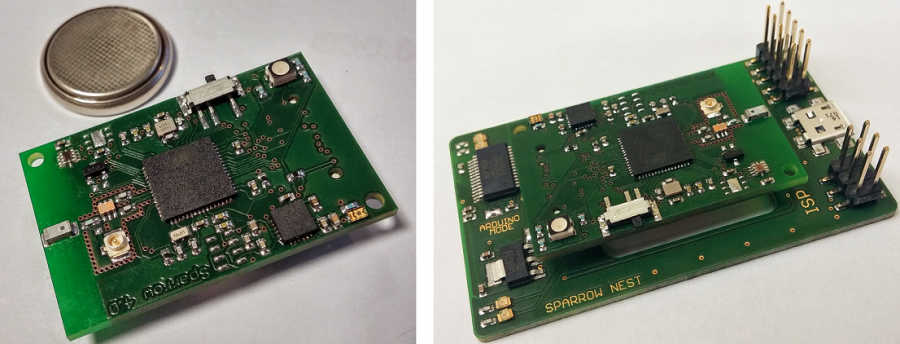
\includegraphics[width=0.5\textwidth]{img/sparrow-v4.png}
  \caption{SparrowV4 wireless sensor nodes}
\end{figure}

\begin{figure}[ht] \centering
  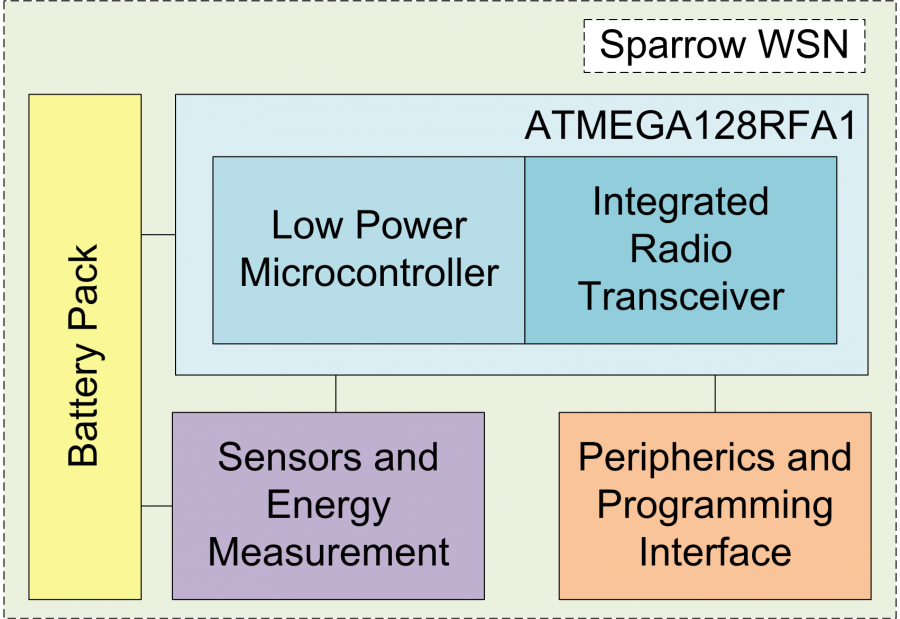
\includegraphics[width=0.5\textwidth]{img/sparrow-v4-arch.png}
  \caption{SparrowV4 hardware architecture}
\end{figure}

In order to monitor its environment, the Sparrow v4 wireless sensor node relies on 3 main sensor peripherals. The first is 
an Si7020 humidity and temperature sensor\cite{Si7020} with incorporated ADC unit. The measurement resolution for relative humidity measurements
can vary between 8 and 12 bits, while the resolution for temperature measurements varies from 11 to 14 bits. The second sensor is 
an MPL3115A2 \cite{MPL3115A2} altimeter which can measure pressure and altitude. This sensor also has an incorporated ADC unit and can measure 
both altitude and pressure with a precision of up to 20 bits. The final sensor mounted on the Sparrow v4 and the most important for 
earthquake and vibration monitoring is the LSM9DS0 IMU(Inertial Measurement Unit)\cite{LSM9DS0}. This chip has 3 channels for linear acceleration measurement, 
3 channels for angular rate measurement and another 3 channels for magnetic field measurement. All data measurements are performed at a 
16 bit resolution. From this last sensor, the metric used by the presented application is the linear acceleration (measured in Gs).
All of the aforementioned sensors are connected to the microcontroller via a two-wire interface. Each of the has a different slave address so 
it is possible for the master, the ATmega128RFA1 controller, to communicate with all of them without interference from the others.

\begin{figure}[ht] \centering
  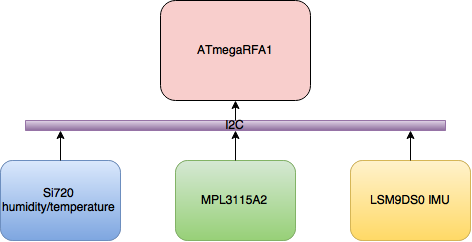
\includegraphics[width=0.5\textwidth]{img/i2c-conn.png}
  \caption{Sensors connected on two-wire interface}
\end{figure}

All the components on the Sparrow v4 node function at a maximum supply voltage of 3.3V. The node can be powered in 2 ways: either from a lithium polymer battery 
cell or via an USB port. When powered via USB, a linear DC regulator is used to drop the supply voltage from the 5V of the USB line to the necessary 3.3V.

The nodes can be easily programmed from a computer using the specially designed programming interface. This interface represents a separate piece of hardware
on which the Sparrow nodes can me mounted. The programming board is built using an FTDI chip which can transform RS-232 transmissions to USB signals. This means 
that the nodes can be programmed using a normal USB connection and no other special programming cable or component is required.

\subsection{Software}

The Sparrow v4 wireless sensor nodes run an Arduino\cite{arduino} compatible firmware. This allows the programmer to easily import 
and use open source Arduino modules for each peripheral. Another advantage of using an Arduino compatible firmware is that it ensures the code is 
compatible with multiple platforms and can be easily modified, upgraded or ported to similar hardware. For development, the Arduino IDE is used 
because it provides access to predefined libraries for peripherals such as serial line, two-wire interface and ADC. It is also available on a wide 
variety of operating systems which makes code modifications and firmware updates easier to implement.

The firmware which runs on the Sparrow v4 nodes operates in two steps. The first step is a calibration phase, which starts running when the sensor 
is first turned on. This will determine the default values for each of the 3 accelerometer axes for the current position of the node. Once this step 
is completed, the node enters its second step in which it will continuously function until it is turned off. During this period, it harvests data 
from the accelerometer and sends it towards a designated gateway. The gateway shall always be connected to a server 
which is capable of plotting and analysing the data. The gateway communicates with this server by means of a serial interface.

\begin{figure}[ht] \centering
  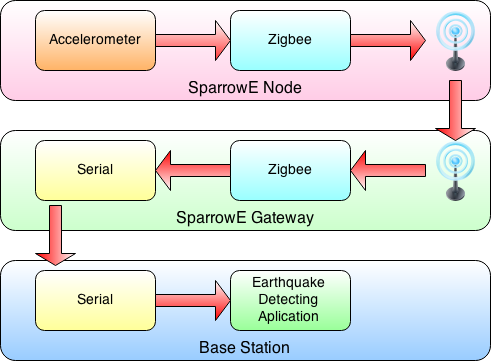
\includegraphics[width=0.5\textwidth]{img/software-architecture.png}
  \caption{Software architecture connections}
\end{figure}

The accelerometer on the Sparrow v4 node is configured for a +/-2G linear acceleration rate and operates at an Ouput Data Rate of 50 Hz. 
The raw data from the 3 axes is translated by the ATmega128RFA1 microcontroller into gravitational scale and then is normalized.

This approach will generate a value of 1G when the node is kept still, in its calibrated position. When the surface starts vibrating, the value will start varying 
above or bellow the reference value of 1G. The calculated data is gathered in sent periodically by the controller to the 
gateway. Node identification data is also added to the sent packets. The gateway is able to collect data from multiple nodes and send it to the base station through
the aforementioned serial connection, which is configured at a baud rate of 1Mbps. The base station is responsible for saving and interpreting the data. 
It is considered that a node has detected an earthquake if the values oscillate strongly over the 1G reference value, reaching peaks at 2G+.

\subsection{Low Power}

The goal of the sensors is to monitor earthquakes and similar phenomena over prolonged periods of time. We must ensure that the Sparrow v4 sensors function in a low power
state and capable of running for prolonged periods of time. This problem is tackled mainly at the software level. At the hardware level, while the components of the sensor 
are selected with regard to power consumption, their power consumption is still relatively high considering the target autonomy of the Sparrow v4 sensor.

In order to overcome this, the firmware is designed to keep the controller in a sleep state and wake it up periodically to read the accelerometer data. 
This technique is similar to clock gating and it is done with the use of a RTC (Real Time Clock). The AtmegRFA1 controller on the nodes offers the ability of using the Timer/Counter2 
peripheral as a real time clock source with an external 32768hz crystal oscillator. The reason why a real time clock is used to implement this mechanism is that even while the controller 
is in sleep mode, this peripheral is still active and it will generate interrupts at certain time intervals, as configured by the programmer. When the controller receives such an 
interrupt, it will wake up and perform any designated operation after which it is put back to sleep and the entire process starts again.

By using this technique, the data from the accelerometer is read and sent to a base station once every half of second instead of once every hundred milliseconds. By doing this, 
the battery is preserved for much longer, as the controller and the transceiver operate for shorter periods of time. The only component with 100 percent uptime is the 
accelerometer. According to the datasheet of each individual component, the accelerometer's consumption in normal mode is 350 micro amps, while the ATmegaRFA1's consumption is
4.7 milli amps in normal mode and 0.2 micro amps in sleep mode. In theory, the sensors should never have  an average power consumption higher the 1 milli amp. An example of the actual power consumption over the course of 1.1 seconds of activity can be seen in figure \ref{power}.

\begin{figure}[ht] \centering
  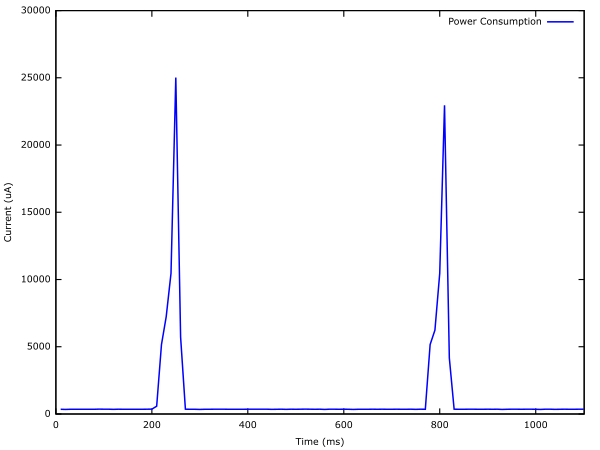
\includegraphics[width=0.5\textwidth]{img/power-graph.png}
  \caption{Power consumption example}
  \label{power}
\end{figure}

While the controller is put into a sleep state, the accelerometer is always powered on and functioning. The LSM9DS0 chip comes with 192 bytes of memory where it can store the data it reads. This allows the controller to always read the latest data from the accelerometer while relaying the oldest to the base-station. Because we use a 50Hz ODR for the accelerometer, the FIFO queue will fill in less then a second. So every other 500 milliseconds we read the data from the FIFO buffer, we process it and send the normalized values to the base station. By doing so, the sensor nodes will be prompt when it comes to detecting events but, at the same time, they will maintain a low power state by transmitting data in smaller quantities over longer periods of time.

With this approach, we increase the autonomy of the Sparrow v4 sensor node while, at the same time, making data easier to handle by the plotting and interpretation software running 
on the base station.
